\documentclass[10pt,booklet]{worship}

\usepackage{amssymb}
\usepackage{multicol}
\usepackage{yfonts}

\begin{document}
  \clearpage
  \vspace*{\fill}

  \begin{center}
    \Huge
    \maltese
    \hspace{1em}
    Tenebræ
    \hspace{1em}
    \maltese
  \end{center}

  \vfill

  \begin{center}
    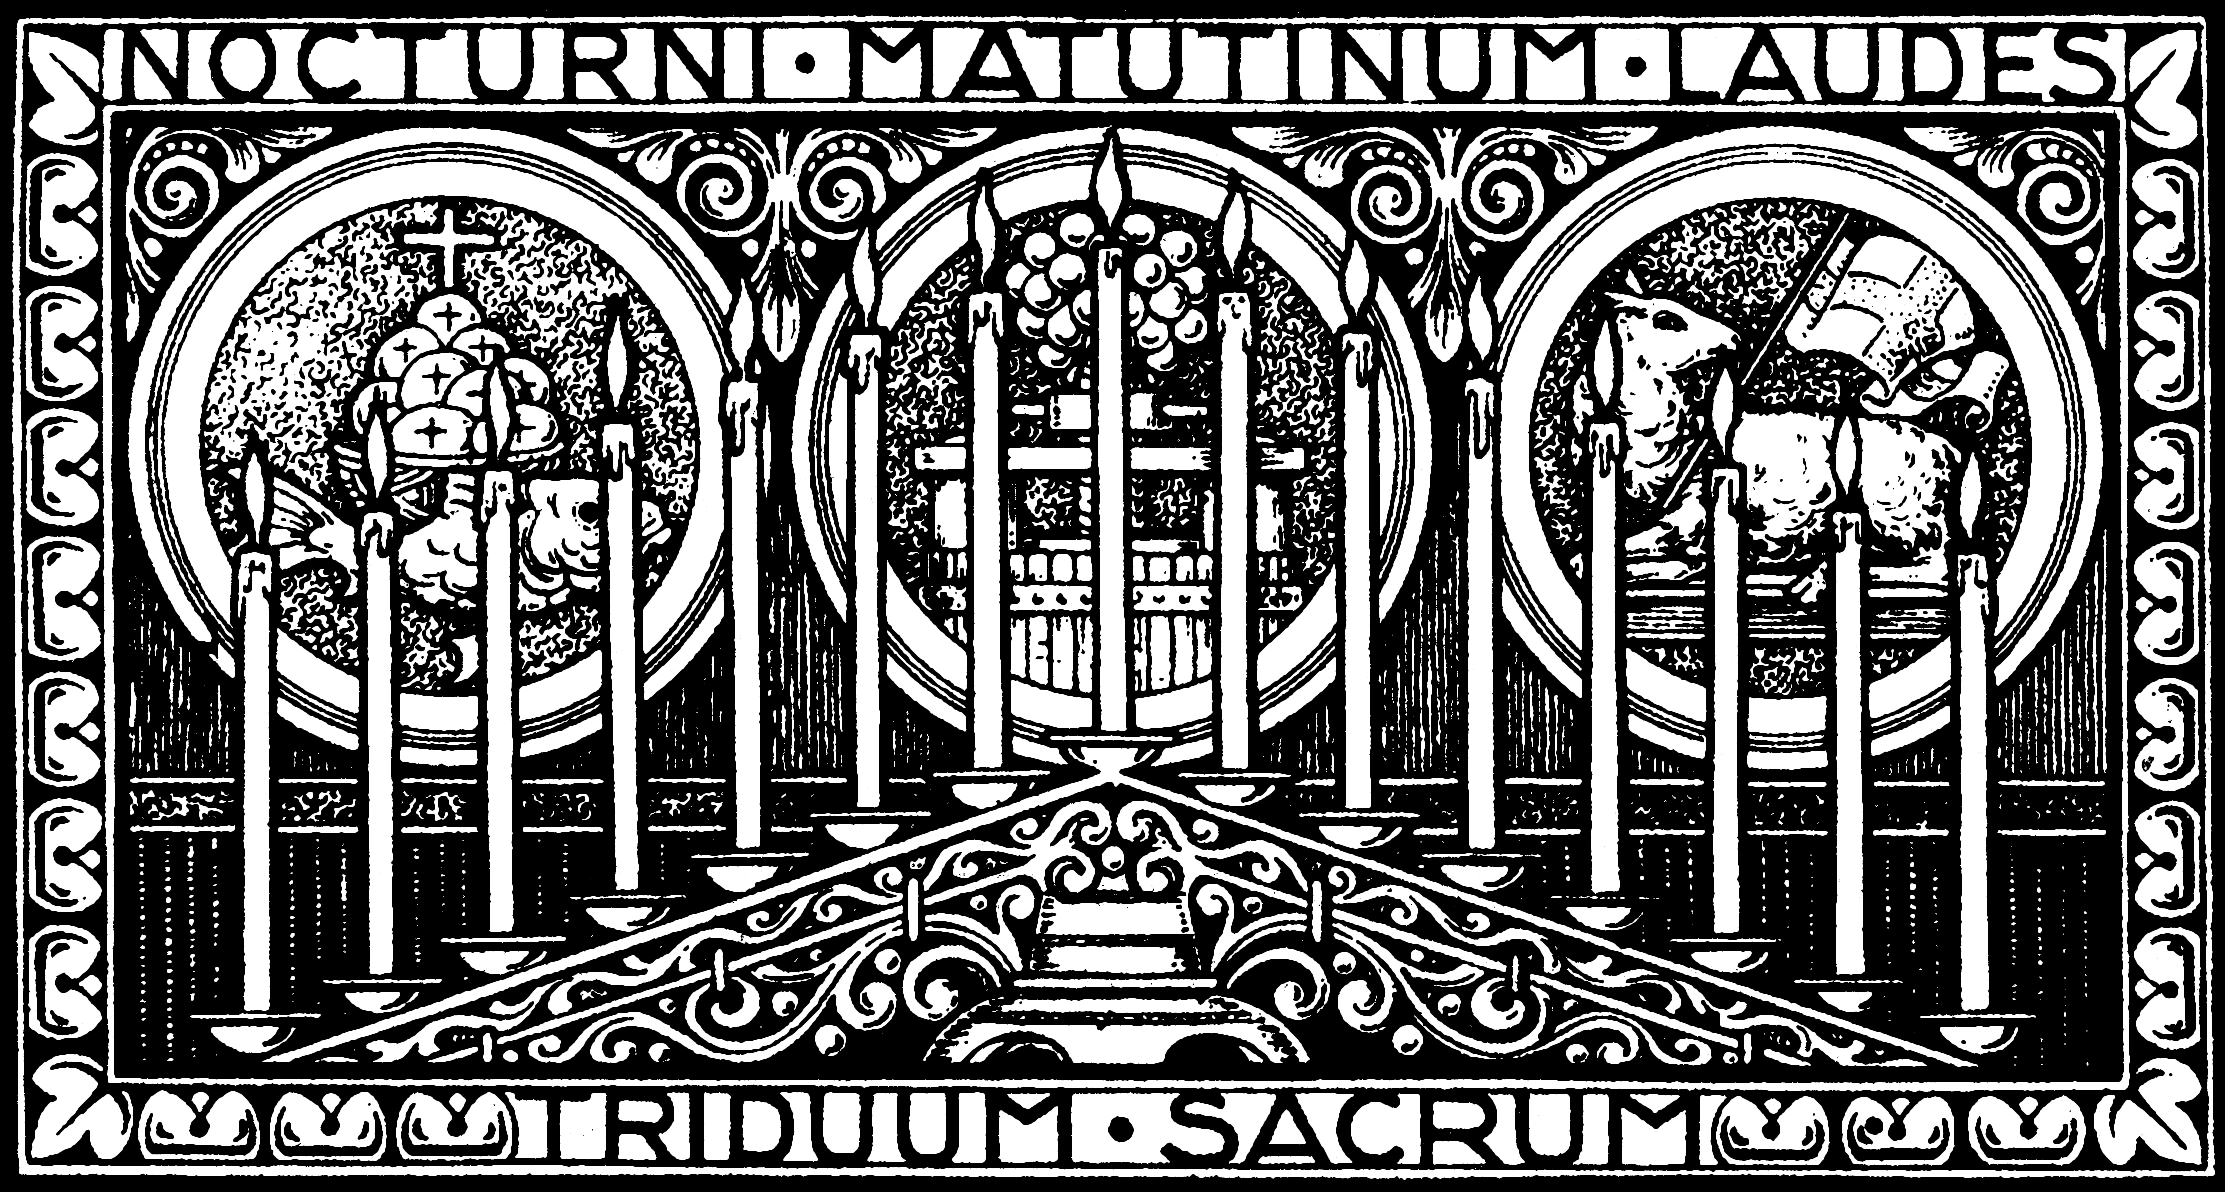
\includegraphics[width=\linewidth]{images/tenebrae.png}
  \end{center}

  \vfill

  \textbf{Tenebræ} is Latin for \emph{darkness} or \emph{shadows}. The Tenebræ
  service, which dates from the Middle Ages, recreates the emotional aspects of
  the Passion. With each read verse, a candle is extinguished. The Lord's Prayer
  is recited. It ends in darkness and with a great noise (the ``Strepitus'') that
  signifies that closing of the Tomb and the tumult in Heaven. Silence follows
  and the people leave under low light.

  \section*{Abbreviations}

  \begin{multicols}{2}
    {\Vbar} = Priest's verse \\
    \textbf{{\Rbar} = Response by all} \\
    C = Cantor

    \columnbreak

    1 = Side 1 (priest's side) \\
    2 = Side 2
  \end{multicols}

  \vfill
  \clearpage

  \section*{Procession}

  \begin{rubric}
    Stand.
  \end{rubric}

  \grechangestaffsize{15}
  \gresetinitiallines{1}
  \gregorioscore{00-procession}

  \tr{\small
    Darkness fell when the Jews crucified Jesus: and about the ninth hour Jesus
    cried with a loud voice: My God, my God, why have you forsaken me? And he
    bowed his head and gave up his spirit. Jesus cried with a loud voice and
    said, Father, into your hands I commend my spirit. And he bowed his head
    and gave up His spirit.
  }

  \begin{versicle}
    \Vbar. Glory be to the Father, to the Son, and to the Holy Spirit.
  \end{versicle}

  \begin{response}
    \Rbar. As it was in the beginning, is now, and ever shall be, world without
    end. Amen.
  \end{response}

  \begin{versicle}
    \Vbar. The Lord be with you.
  \end{versicle}

  \begin{response}
    \Rbar. And with your spirit.
  \end{response}

  \begin{versicle}
    \Vbar. Almighty and ever-living God, who as an example of humility for the
    human race to follow caused our Savior to take flesh and submit to the Cross,
    graciously grant that we may heed his lesson of patient suffering and so
    merit a share in his Resurrection. Who lives and reigns with you in the unity
    of the Holy Spirit, one God for ever and ever.
  \end{versicle}

  \begin{response}
    \Rbar. Amen.
  \end{response}

  \begin{rubric}
    Sit.

    The first candle is extinguished.
  \end{rubric}

  \section*{Psalm 51}

  \grechangestaffsize{13}
  \gresetinitiallines{1}
  \gregorioscore{01-psalm51}

  \vspace{1.5em}

  1. Wash away all my guilt; from my sin cleanse me. For I know my offense; my
  sin is always before me. Against you alone have I sinned; I have done such evil
  in your sight that you are just in your sentence, blameless when you condemn.
  \Rbar.

  2. True, I was born guilty, a sinner, even as my mother conceived me. Still,
  you insist on sincerity of heart; in my inmost being teach me wisdom. Cleanse
  me with hyssop, that I may be pure; wash me, make me whiter than snow. Let me
  hear sounds of joy and gladness; let the bones you have crushed rejoice. \Rbar.

  1. Turn away your face from my sins; blot out all my guilt. A clean heart
  create for me, God; renew in me a steadfast spirit. Do not drive me from your
  presence, nor take from me your holy spirit. Restore my joy in your salvation;
  sustain in me a willing spirit. \Rbar.

  2. I will teach the wicked your ways, that sinners may return to you. Rescue me
  from death, God, my saving God, that my tongue may praise your healing power.
  {\Lord}, open my lips; my mouth will proclaim your praise. For you do not desire
  sacrifice; a burnt offering you would not accept. \Rbar.

  1. My sacrifice, God, is a broken spirit; God, do not spurn a broken, humbled
  heart. Make Zion prosper in your good pleasure; rebuild the walls of Jerusalem.
  Then you will be pleased with proper sacrifice, burnt offerings and holocausts;
  then bullocks will be offered on your altar. \Rbar.

  \begin{rubric}
    The second candle is extinguished.
  \end{rubric}

  \clearpage

  \section*{Psalm 63}

  \grechangestaffsize{13}
  \gresetinitiallines{1}
  \gregorioscore{02-psalm63}

  \vspace{1.5em}

  1. For you my body yearns; for you my soul thirsts, Like a land parched,
  lifeless, and without water. So I look to you in the sanctuary to see your
  power and glory. For your love is better than life; my lips offer you worship!
  \Rbar.

  2. I will bless you as long as I live; I will lift up my hands, calling on your
  name. My soul shall savor the rich banquet of praise, with joyous lips my mouth
  shall honor you! When I think of you upon my bed, through the night watches I
  will recall that you indeed are my help, and in the shadow of your wings I
  shout for joy. \Rbar.

  1. My soul clings fast to you; your right hand upholds me. But those who seek
  my life will come to ruin; they shall go down to the depths of the earth! They
  shall be handed over to the sword and become the prey of jackals! But the king
  shall rejoice in God; all who swear by the {\Lord} shall exult, for the mouths of
  liars will be shut! \Rbar.

  \begin{rubric}
    The third candle is extinguished.
  \end{rubric}

  \section*{Psalm 27}

  \grechangestaffsize{13}
  \gresetinitiallines{1}
  \gregorioscore{03-psalm27}

  \vspace{1.5em}

  1. The {\Lord} is my life's refuge; of whom am I afraid? When evildoers come at me
  to devour my flesh, these my enemies and foes themselves stumble and fall. \Rbar.

  2. Though an army encamp against me, my heart does not fear; Though war be
  waged against me, even then do I trust. But I believe I shall enjoy the {\Lord}'s
  goodness in the land of the living. Wait for the {\Lord}, take courage; be
  stouthearted, wait for the {\Lord}! \Rbar.

  \begin{rubric}
    The fourth candle is extinguished.
  \end{rubric}

  \clearpage

  \section*{Miserere Mei}

  \begin{rubric}
    Choir stand.
  \end{rubric}

  \grechangestaffsize{15}
  \gresetinitiallines{1}
  \gregorioscore{04-miserere-mei}
  \begin{flushright}
    \tr{\small
      Have mercy on me, God, according to your great mercies.
    }
  \end{flushright}

  \begin{rubric}
    The fifth candle is extinguished.
  \end{rubric}

  \section*{Reading I: Isaiah 42}

  1. Here is my servant whom I uphold, my chosen one with whom I am pleased, upon
  whom I have put my spirit; he shall bring forth justice to the nations, Not
  crying out, not shouting, not making his voice heard in the street.

  2. A bruised reed he shall not break, and a smoldering wick he shall not
  quench, until he establishes justice on the earth; the coastlands will wait for
  his teaching.

  1. Thus says God, the {\Lord}, who created the heavens and stretched them out, who
  spreads out the earth with its crops, who gives breath to its people and
  spirit to those who walk on it:

  2. I, the {\Lord}, have called you for the victory of justice, I have grasped you
  by the hand; I formed you, and set you as a covenant of the people, a light for
  the nations,

  1. To open the eyes of the blind, to bring out prisoners from confinement, and
  from the dungeon, those who live in darkness.

  \grechangestaffsize{13}
  \gresetinitiallines{0}
  \gregorioscore{vd5}
  \begin{flushright}
    \tr{\small
      C. The word of the Lord.
      \textbf{\Rbar. Thanks be to God.}
    }
  \end{flushright}

  \begin{rubric}
    The sixth candle is extinguished.
  \end{rubric}

  \section*{Reading II: Lamentations 3}

  1. I am a man who knows affliction from the rod of his anger, one whom he has
  led and forced to walk in darkness, not in the light; against me alone he
  brings back his hand again and again all the day.

  2. He has worn away my flesh and my skin, he has broken my bones; He has beset
  me round about with poverty and weariness; He has left me to dwell in the dark
  like those long dead.

  1. He has hemmed me in with no escape and weighed me down with chains; even
  when I cry out for help, he stops my prayer; He has blocked my ways with fitted
  stones, and turned my paths aside.

  2. He has broken my teeth with gravel, pressed my face in the dust; My soul is
  deprived of peace, I have forgotten what happiness is; I tell myself my future
  is lost, all that I hoped for from the {\Lord}.

  1. But I will call this to mind, as my reason to have hope: The favors of the
  {\Lord} are not exhausted, his mercies are not spent; they are renewed each
  morning, so great is his faithfulness.

  2. My portion is the {\Lord}, says my soul; therefore will I hope in him. Good is
  the {\Lord} to one who waits for him, to the soul that seeks him; it is good to
  hope in silence for the saving help of the {\Lord}.

  1. It is good for a man to bear the yoke from his youth. Let him sit alone and
  in silence, when it is laid upon him. Let him put his mouth to the dust; there
  may yet be hope. Let him offer his cheek to be struck, let him be filled with
  disgrace. For the {\Lord}'s rejection does not last forever;

  \grechangestaffsize{13}
  \gresetinitiallines{0}
  \gregorioscore{vd3}
  \begin{flushright}
    \tr{\small
      C. The word of the Lord.
      \textbf{\Rbar. Thanks be to God.}
    }
  \end{flushright}

  \begin{rubric}
    The seventh candle is extinguished.
  \end{rubric}

  \section*{Reading III: Lamentations 5}

  1. Remember, O {\Lord}, what has befallen us, look, and see our disgrace: Our
  inherited lands have been turned over to strangers, our homes to foreigners.

  2. We have become orphans, fatherless; widowed are our mothers. The water we
  drink we must buy, for our own wood we must pay. On our necks is the yoke of
  those who drive us; we are worn out, but allowed no rest.

  1. To Egypt we submitted, and to Assyria, to fill our need of bread. Our
  fathers, who sinned, are no more; but we bear their guilt. Slaves rule over us;
  there is no one to rescue us from their hands.

  2. At the peril of our lives we bring in our sustenance, in the face of the
  desert heat; our skin is shriveled up, as though by a furnace, with the searing
  blasts of famine.

  1. The old men have abandoned the gate, the young men their music. The joy of
  our hearts has ceased, our dance has turned into mourning; the garlands have
  fallen from our heads: woe to us, for we have sinned!

  2. Over this our hearts are sick; at this our eyes grow dim: That Mount Zion
  should be desolate, with jackals roaming there! You, O {\Lord}, are enthroned
  forever; your throne stands from age to age.

  1. Why, then, should you forget us, abandon us so long a time? Lead us back to
  you, O {\Lord}, that we may be restored: give us anew such days as we had of old.

  \grechangestaffsize{13}
  \gresetinitiallines{0}
  \gregorioscore{vd5}
  \begin{flushright}
    \tr{\small
      C. The word of the Lord.
      \textbf{\Rbar. Thanks be to God.}
    }
  \end{flushright}

  \begin{rubric}
    The eighth candle is extinguished.
  \end{rubric}

  \section*{Psalm 69}

  \grechangestaffsize{11}
  \gresetinitiallines{1}
  \gregorioscore{05-psalm69}

  \vspace{1.5em}

  1. Do not hide your face from your servant; in my distress hasten to answer me.
  Come and ransom my life; because of my enemies redeem me. \Rbar.

  2. You know my reproach, my shame, my disgrace; before you stand all my foes.
  Insult has broken my heart, and I am weak; I looked for compassion, but there
  was none, for comforters, but found none. \Rbar.

  1. Instead they put gall in my food; for my thirst they gave me vinegar. I am
  afflicted and in pain; let your saving help protect me, God, that I may praise
  God's name in song and glorify it with thanksgiving. \Rbar.

  \begin{rubric}
    The ninth candle is extinguished.
  \end{rubric}

  \section*{Psalm 38}

  \grechangestaffsize{13}
  \gresetinitiallines{1}
  \gregorioscore{06-psalm38}

  \vspace{1.5em}

  1. O {\Lord}, do not rebuke me in your anger; do not punish me, {\Lord}, in your
  rage. Your arrows have sunk deep in me; your hand has come down upon me.
  Through your anger all my body is sick: through my sin, there is no health in
  my limbs. \Rbar.

  2. My guilt towers higher than my head; it is a weight too heavy to bear. My
  wounds are foul and festering, the result of my own folly. I am bowed and
  brought to my knees. I go mourning all the day long. \Rbar.

  1. All my frame burns with fever; all my body is sick. Spent and utterly
  crushed, I cry aloud in anguish of heart. O {\Lord}, you know all my longing: my
  groans are not hidden from you. My heart throbs, my strength is spent; the very
  light has gone from my eyes. \Rbar.

  2. For I am on the point of falling and my pain is always before me. I confess
  that I am guilty and my sin fills me with dismay. My wanton enemies are
  numberless and my lying foes are many. They repay me evil for good and attack
  me for seeking what is right. \Rbar.

  1. O {\Lord}, do not forsake me! My God, do not stay afar off! Make haste and come
  to my help, O {\Lord}, my God, my savior! \Rbar.

  \begin{rubric}
    The tenth candle is extinguished.
  \end{rubric}

  \section*{Parce Domine}

  \begin{rubric}
    Choir stand.
  \end{rubric}

  \grechangestaffsize{15}
  \gresetinitiallines{1}
  \gregorioscore{07-parce-domine}

  \begin{flushright}
    \tr{\small
      Spare, Lord, spare your people:
      Be not angry with us forever.
    }
  \end{flushright}

  \begin{rubric}
    The eleventh candle is extinguished.
  \end{rubric}

  \section*{Reading IV: Isaiah 52--53}

  \begin{rubric}
    Canticle of the Suffering Servant
  \end{rubric}

  1. My servant shall prosper, he shall be raised high and greatly exalted. Even
  as many were amazed at him---so marred was his look beyond that of man, and his
  appearance beyond that of mortals.

  2. So shall he startle many nations, because of him kings shall stand
  speechless; For those who have not been told shall see, those who have not
  heard shall ponder it.

  1. Therefore I will give him his portion among the great, and he shall divide
  the spoils with the mighty, because he surrendered himself to death and was
  counted among the wicked; and he shall take away the sins of many, and win
  pardon for their offenses.

  \grechangestaffsize{13}
  \gresetinitiallines{0}
  \gregorioscore{vd3}
  \begin{flushright}
    \tr{\small
      C. The word of the Lord.
      \textbf{\Rbar. Thanks be to God.}
    }
  \end{flushright}

  \begin{rubric}
    The twelfth candle is extinguished.
  \end{rubric}

  \section*{O Vos Omnes}

  \begin{rubric}
    Choir stand.
  \end{rubric}

  \begin{multicols}{2}
    O vos omnes, \\
    qui transitis per viam, \\
    attendite, et videte \\
    si est dolor similis \\
    sicut dolor meus.

    \columnbreak

    \tr{
      All you \\
      who pass by the way, \\
      look and see \\
      whether there is any sorrow \\
      like my sorrow.
    }
  \end{multicols}

  \begin{rubric}
    The thirteenth candle is extinguished.
  \end{rubric}

  \clearpage

  \section*{Magnificat}

  \begin{rubric}
    Stand.
  \end{rubric}

  Magníficat ánima mea Dóminum, \\
  et exsultávit spíritus meus, in Deo salutári meo, \\
  quia respéxit humilitátem ancíllæ suæ. \\
  Ecce enim ex hoc beátam me dicent omnes generatiónes, \\
  quia fécit mihi mágna, qui pótens est: et sánctum nómen ejus, \\
  et misericórdia ejus a progénie in progénies timéntibus eum. \\
  Fécit poténtiam in bráchio suo, dispérsit supérbos mente cordis sui; \\
  depósuit poténtes de sede et exaltávit húmiles; \\
  esuriéntes implévit bonis et dívites dimísit inánes. \\
  Suscépit Ísraël púerum suum, recordátus misericórdiæ suæ, \\
  sicut locútus est ad patres nostros, Ábraham et sémini ejus in sǽcula. \\
  Glória Patri, et Fílio, et Spirítui Sancto. \\
  Sicut erat in princípio, et nunc, et semper, et in sǽcula sæculórum. Amen.

  \tr{\small
    My soul magnifies the Lord. \\
    And my spirit rejoices in God my Savior \\
    Because He has regarded the humility of His handmaid: \\
    For behold from henceforth all generations shall call me blessed. \\
    Because He that is mighty has done great things to me; and holy is His name. \\
    And His mercy is from generation unto generations, to them that fear Him. \\
    He has shown might in His arm: He has scattered the proud in the conceit of their heart. \\
    He has put down the mighty from their seat, and has exalted the humble. \\
    He has filled the hungry with good things, and the rich He has sent away empty. \\
    He has received Israel His servant, being mindful of His mercy: \\
    As He spoke to our fathers, to Abraham and his children for ever. \\
    Glory be to the Father, and to the Son, and to the Holy Spirit: \\
    As it was in the beginning, is now, and ever shall be, world without end, Amen.
  }

  \begin{rubric}
    The fourteenth candle is extinguished.
  \end{rubric}

  \begin{center}
    \includegraphics[height=1.75in]{images/pieta.png}
  \end{center}

  \clearpage

  \section*{The Lord's Prayer}

  \begin{versicle}
    \Vbar. At the Savior's command and formed by divine teaching, we dare to say:
  \end{versicle}

  \begin{response}
    Our father, who art in heaven, \\
    Hallowed be thy name; \\
    Thy kingdom come; \\
    Thy will be done on earth as it is in heaven. \\
    Give us this day our daily bread; \\
    And forgive us our trespasses \\
    As we forgive those who trespass against us; \\
    And lead us not into temptation, \\
    But deliver us from evil.
  \end{response}

  \section*{Concluding Prayer}

  \begin{versicle}
    \Vbar. Look we pray, O Lord, on this your family, for whom our Lord Jesus
    Christ did not hesitate to be delivered into the hands of the wicked and
    submit to the agony of the Cross. Who lives and reigns with you in the unity
    of the Holy Spirit, one God, for ever and ever.
  \end{versicle}

  \begin{response}
    \Rbar. Amen.
  \end{response}

  \begin{rubric}
    The fifteenth candle is removed.
  \end{rubric}

  % \begin{center}
  %   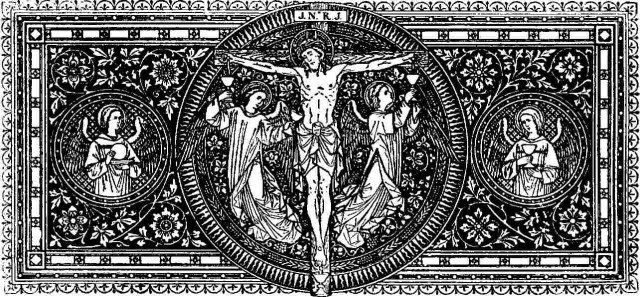
\includegraphics[width=\textwidth]{images/crucifixion.jpg}
  % \end{center}

  % \clearpage

  \section*{The Strepitus}

  \begin{rubric}
    Assembly repeatedly beats the pews with their hands until the fifteenth candle is returned.
  \end{rubric}

  % \begin{center}
  %   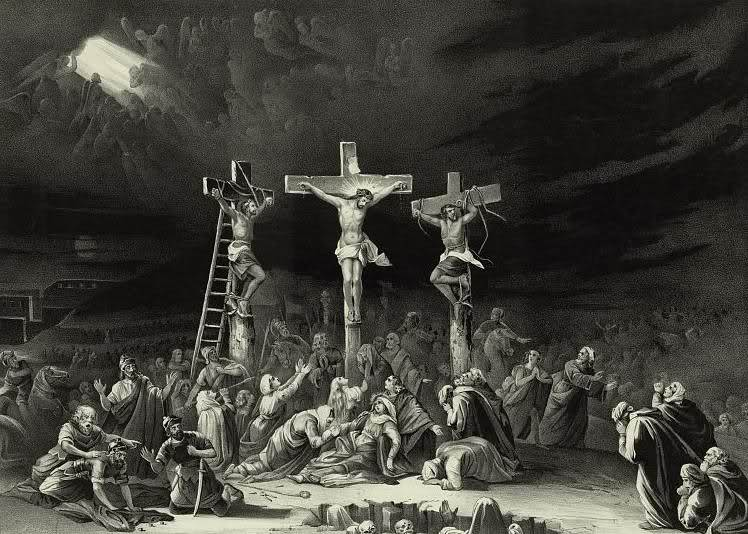
\includegraphics[width=\textwidth]{images/crucifixion-painting.jpg}
  % \end{center}

  \begin{rubric}
    Assembly departs in silence.
  \end{rubric}

  \begin{center}
    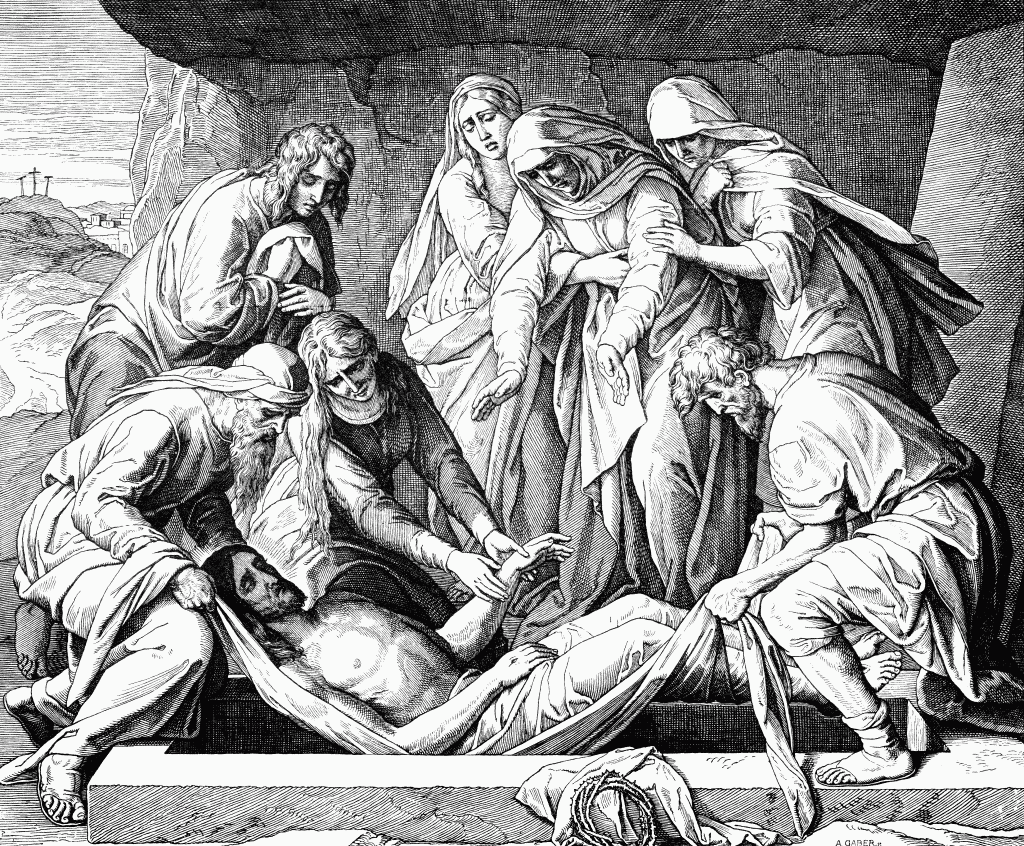
\includegraphics[height=1.75in]{images/burial.png}
  \end{center}

  \vfill

  \begin{center}
    \tiny
    Rev. \today
  \end{center}
\end{document}
